\chapter{Background}
\label{chp:background} 

\section{Village Telco}
%How did it all start?

\section{Mesh Potato}
%Generelt om MP

% hvordan MPen fikk navnet. 

\begin{figure}[h!]
  \centering
      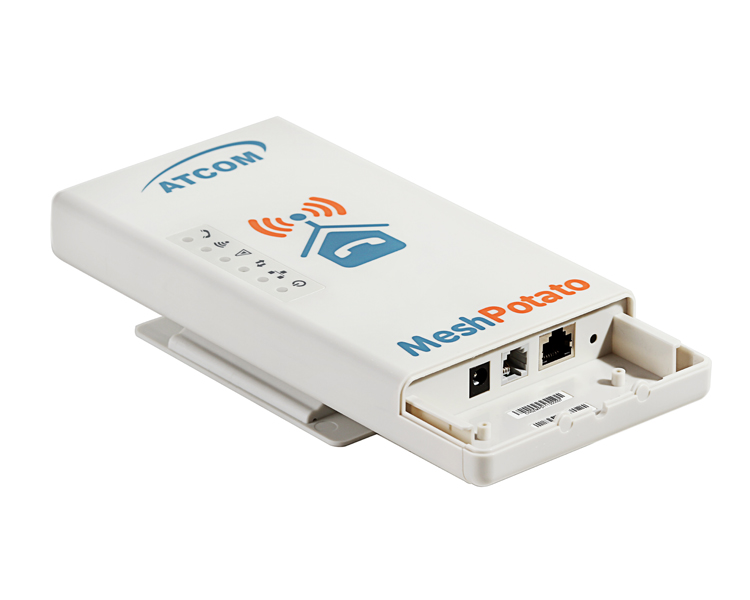
\includegraphics[width=0.5\textwidth]{MP01}
  \caption [The Mesh Potato]{\textbf{The fist generation Mesh Potato, MP01}}
  \label{fig:MP01}
\end{figure}

%MP01
The Mesh Potato, as shown in \fref{MP01}, is designed to be used in rural areas. It can be deplyed and run anywhere in the world relying only on a low, but stable power supply. The ethernet port, Foreign eXchange Station (FXS) ports and power are robust and designed to handle hard weather, poor power conditions, lightening and static electricity. In addition the Mesh Potato comes in a waterproof box for outdoor mounting \cite{background}.

The Mesh Potato combines the features of a 802.11bg WiFi router with an Analog telephone Adaptor (ATA) \cite{MP}. Each Mesh Potato provies a single fixed telephone line to the end user. The MPs are connected together via a mesh WiFi network, and  configure themselves automatically to form a peer-to-peer network, greatly extending the range of the network over regual WiFi. Enabling phone calls to be made independent of landlines and telephone towers. Creating the basis for the "plug-and-play" solution. 








The Mesh network can be connected vi a backbone link to the rest of the world by using VoIP trunks. 


MP02





\section{Technology}

\subsection{Ad Hoc and Mesh Networks}
Mobile ad hoc networks (MANETs) are networks that does not rely on an underlying and fixed infrastructure, in other words infrastructureless. MANETs acts in a shared wireless media \cite{adhoc}. The structure of these networks change dynamically, and key factors for MANETs is self-configuration and self-organization. The members of the network are mobile and are free to join or leave the network \cite{adhoc2}, and therefore these factors are important. MANETs are based on multi-hop forwarding. This means that each node acts not only as a host, but also as a router. The nodes themselves establishes and maintain routes, and forward packets to other nodes if necessary. This enables communication between nodes that are originally not within each other's send range \cite{adhoc2}. Because of these characteristics MANETs is suited for use in situations where there are no fixed underlying infrastructure. MANETs can operate as a stand-alone solution, but it can also be attached to the Internet. This makes room for numerous of services. 

\begin{figure}[h!]
  \centering
    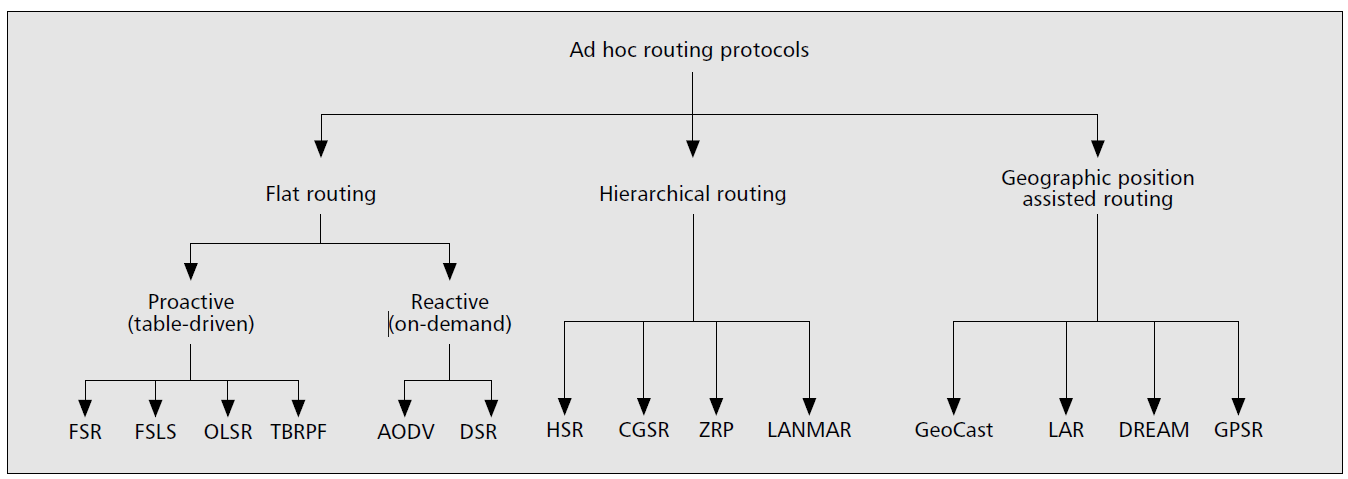
\includegraphics[width=1\textwidth]{adhocprotocols.png}
     \caption{Different groups of ad hoc routing protocols \cite{adhoc}.}
\label{fig:adhoc}
\end{figure}

\paragraph{}
There exists many challenges when it comes to these types of networks. The routing protocols must be able to adapt quickly due to the topology changes. \fref{fig:adhoc} shows the different groups of the ad hoc protocols that exist. The routing protocols must not cause excessive overhead. Under the category flat routing, there are two types of routing protocols; proactive and reactive. \textit{Proactive routing protocols} are table driven \citep{proactivereactive}. This means that every network node has a routing table for the forwarding of data. To obtain stability, each node broadcasts and modifies the routing table periodically. Proactive routing protocols are suitable when there are few nodes in the network. Because of the routing table that is periodically updated, the overhead exceeds the desired value when there are a high number of nodes in the network. In contrary to the proactive routing protocols, \textit{reactive routing protocols} are on demand. Since they are on demand, the overhead is significantly lower. These protocols utilizes flooding, and does not have a up-to-date routing table like proactive routing protocols. Routes are only set up to nodes they communicate with \cite{adhoc2}. These routes are only kept alive while they are needed. 




%Eksempel på nettverk

\subsection{OpenWrt}

\section{The Cost Structure and Revenue Model(s) of Village Telco Today}

\section{Comparison of Village Telco and Other Telcos}

\section{Refugee Camps}
\subsection{The Existing Communication Methods}